% elementos pré-textuais 

% título do sumário
\ifdefined\contentsname
  \renewcommand*\contentsname{SUMÁRIO}
\else
  \newcommand\contentsname{SUMÁRIO}
\fi

% capa 
\imprimircapa

% folha de rosto 
% o * indica que haverá a ficha bibliográfica 
\imprimirfolhaderosto*

% ficha catalográfica 
%\begin{fichacatalografica}
%    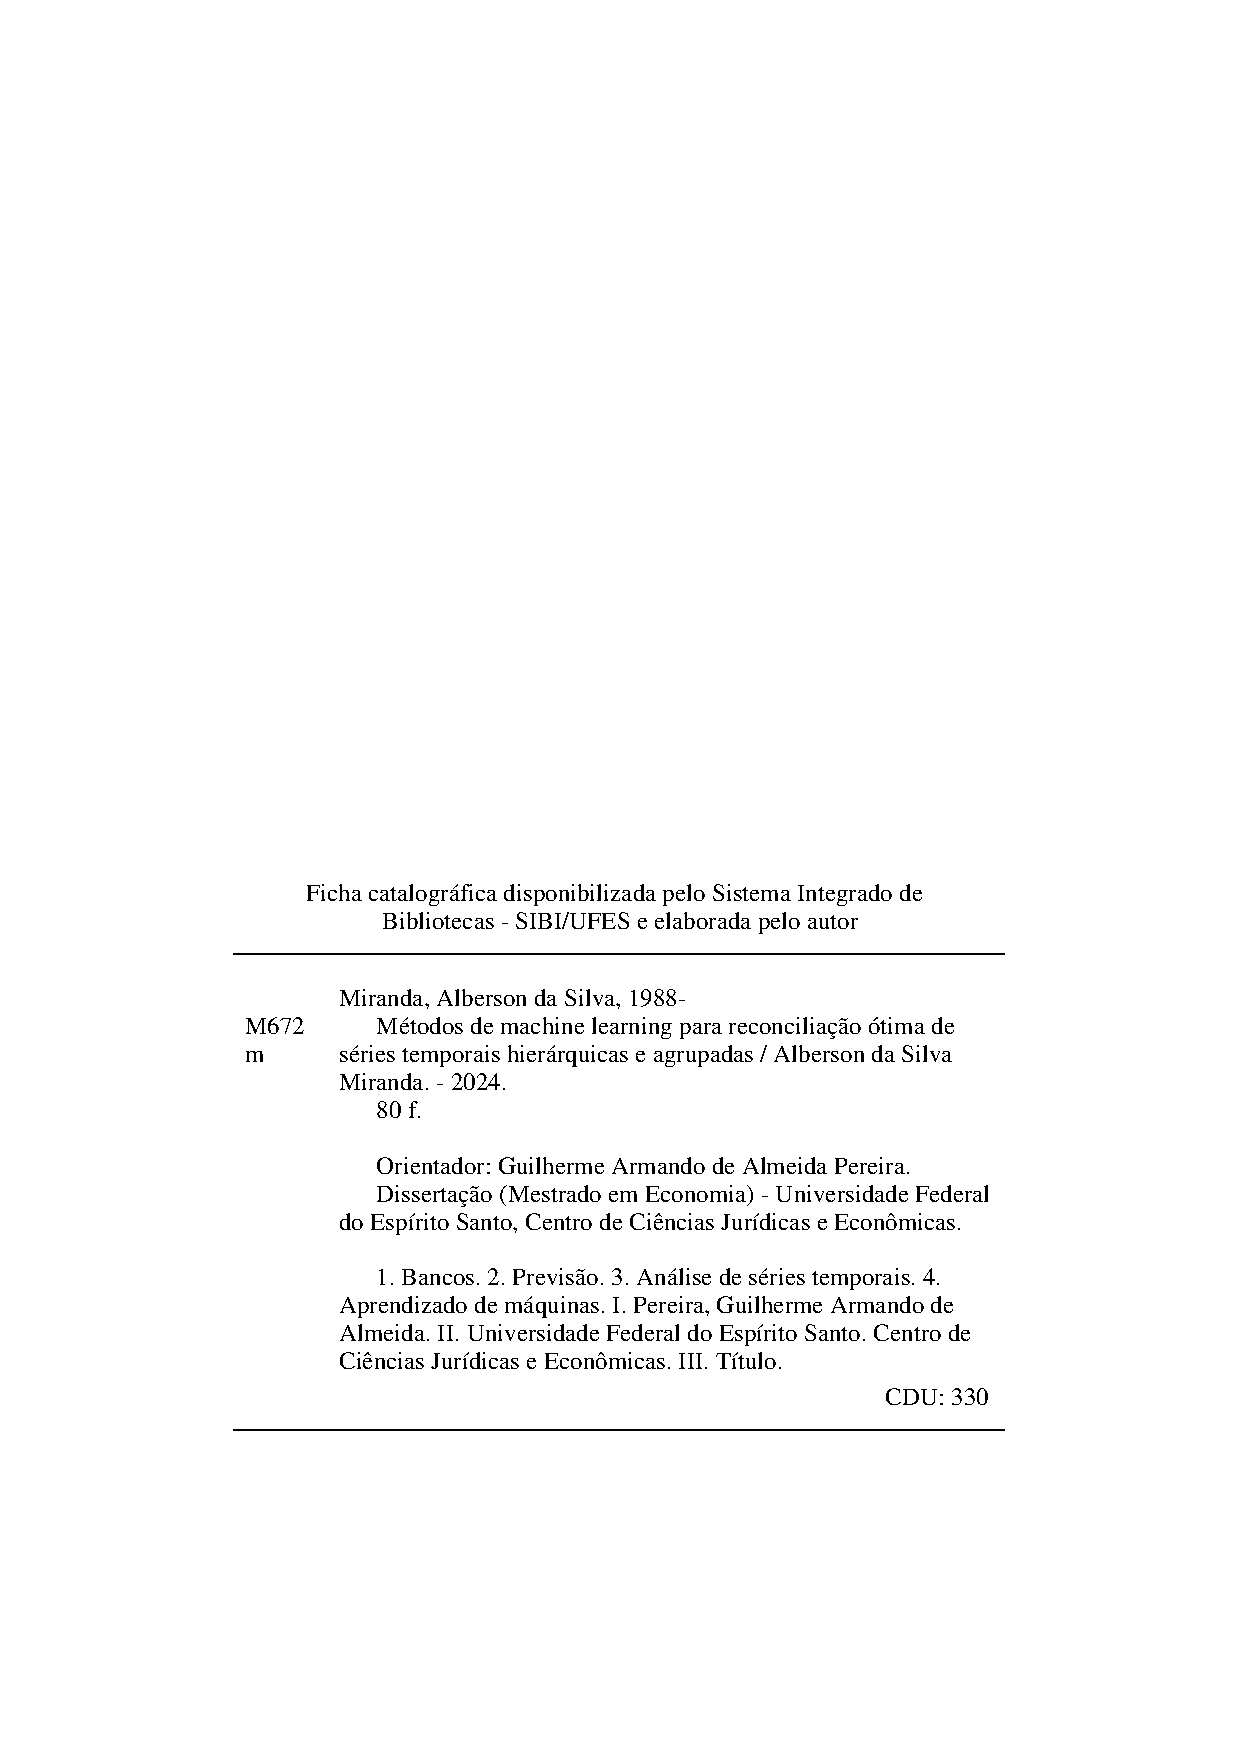
\includepdf{ficha_ufes.pdf}
%\end{fichacatalografica}


% substituir pela ficha em pdf fornecida pela UFES após defesa 
\begin{fichacatalografica}
	\sffamily
	\vspace*{\fill}					% Posição vertical
	\begin{center}					% Minipage Centralizado
	\fbox{\begin{minipage}[c][8cm]{15cm}		% Largura
	\small
	\imprimirautor
	
	\hspace{0.5cm} \imprimirtitulo  / \imprimirautor. --
	\imprimirlocal, \imprimirdata-
	
	\hspace{0.5cm} \thelastpage p. : il. (algumas color.) ; 30 cm.\\
	
	\hspace{0.5cm} \imprimirorientadorRotulo~\imprimirorientador\\
	
	\hspace{0.5cm}
	\parbox[t]{\textwidth}{\imprimirtipotrabalho~--~\imprimirinstituicao,
	\imprimirdata.}\\
	
	\hspace{0.5cm}
		1. Economia Bancária.
		2. Séries Temporais Hierárquicas.
		3. Reconciliação Ótima.
    4. Machine Learning.
		I. Pereira, Guilherme Armando de Almeida.
		II. Universidade Federal do Espírito Santo.
		III. Centro de Ciências Jurídicas e Econômicas.
		IV. Título 			
	\end{minipage}}
	\end{center}
\end{fichacatalografica}

% folha de aprovação 
%
%\begin{folhadeaprovacao}
%    \includepdf{folhadeaprovacao_final.pdf}
%\end{folhadeaprovacao}


% substituir pela folha assinada pela banca após defesa 
\begin{folhadeaprovacao}

  \begin{center}
    {\ABNTEXchapterfont\large\imprimirautor}

    \vspace*{\fill}\vspace*{\fill}
    \begin{center}
      \ABNTEXchapterfont\bfseries\Large\imprimirtitulo
    \end{center}
    \vspace*{\fill}
    
    \hspace{.45\textwidth}
    \begin{minipage}{.5\textwidth}
        \imprimirpreambulo
        \vspace*{1cm}
        Aprovada em 29 de fevereiro de 2024.\\[2cm]
        \textbf{COMISSÃO EXAMINADORA} \\
        \assinatura{\textbf{\imprimirorientador} \\ Universidade Federal do Espírito Santo \\ Orientador} 
        \assinatura{\textbf{Prof. Dr. Edson Zambon Monte} \\ Universidade Federal do Espírito Santo}
        \assinatura{\textbf{Prof. Dr. Fernando Luiz Cyrino Oliveira} \\ PUC-Rio}
        %\assinatura{\textbf{Professor} \\ Convidado 3}
        %\assinatura{\textbf{Professor} \\ Convidado 4}
    \end{minipage}%
   \end{center}
  
\end{folhadeaprovacao}

%% dedicatória 
%\begin{dedicatoria}
%   \vspace*{\fill}
%   \centering
%   \noindent
%   \textit{Exemplo de dedicatória,\\\lipsum[10].} \vspace*{\fill}
%\end{dedicatoria}

%% agradecimentos 
\begin{agradecimentos}
  A jornada para a conclusão do mestrado não poderia ter sido tão gratificante e enriquecedora sem a influência de várias pessoas. Primeiramente, gostaria de expressar minha profunda gratidão ao meu orientador, Dr. Guilherme Pereira, por sua orientação, gentileza e encorajamento constante ao longo de todo o processo. Sua paciência e dedicação foram essenciais para transformar este aluno confuso em um pesquisador.

  À banca examinadora, aos professores Dr. Edson Zambon e Dr. Fernando Cyrino, gostaria de agradecer por aceitarem o convite (mesmo que em curto prazo) para avaliar este trabalho e por fornecerem suas percepções valiosas que aprimoraram e ressignificaram minha pesquisa.

  Ao corpo docente do PPGEco/UFES, em especial meus professores Dr. Edson Zambon, cuja meticulosidade e entrega, aula após aula, desde a graduação, foram determinantes tanto na minha vida acadêmica quanto profissional, e ao Dr. Alain Herscovici, pelas inúmeras conversas, da música à filosofia, da sociologia à epistemologia, que enriqueceram minha perspectiva e ampliaram meus horizontes.

  Agradeço também aos Dr. Nikolaos Kourentzes e Dr. Evangelos Spiliotis por suas contribuições à literatura de previsão hierárquica, que serviram de inspiração para o meu trabalho. Sua generosidade em responder às minhas perguntas e compartilhar dados e códigos foi fundamental para o progresso da minha pesquisa.

  Aos meus professores do curso de matemática do Ifes/Vitória, em particular aos professores Diogo Oliveira, Débora Domingues e Lourenço Gonçalves, expresso minha gratidão pelas conversas e pelo incentivo constante ao longo desta jornada acadêmica.

  Aos meus colegas do programa, Dreyfuss, Yasmin (obrigado pelas revisões!), Amanda, Leina, Ricardo, Michelle e Eduardo, agradeço pela troca de experiências, pelo apoio mútuo e pela camaradagem durante todo o período do mestrado.

  E o mais importante, à minha família, Regina, Aldo, Rafaela e minhas sobrinhas, por todo o apoio e amor incondicional. Tem sido uma jornada. Obrigado por estarem ao meu lado.
\end{agradecimentos}

% epígrafe 
%\begin{epigrafe}
%    \vspace*{\fill}
%	\begin{flushright}
%		\textit{``Modelo de epígrafe, \\
%		modelo de epígrafe.''}
%	\end{flushright}
%\end{epigrafe}

% resumo 

\setlength{\absparsep}{18pt}
\begin{resumo}
  Na última década, a previsão de séries temporais hierárquicas experimentou um crescimento substancial, caracterizado por avanços que melhoraram significativamente a precisão dos modelos de previsão. Recentemente, os métodos de \textit{machine learning} foram integrados à literatura de previsão hierárquica como uma nova abordagem para a reconciliação de previsões. Este trabalho se baseia nesses avanços, explorando ainda mais o potencial dos métodos de \textit{machine learning} para otimizar a reconciliação de séries temporais hierárquicas e agrupadas. Além disso, investigamos o impacto de várias estratégias de aquisição de conjuntos de treinamento, como previsões obtidas por \textit{rolling forecasting}, valores ajustados de modelos reestimados e valores ajustados dos modelos de previsão base, como também estratégias alternativas de validação cruzada. Para avaliar a metodologia proposta, dois estudos de caso foram realizados. O primeiro estudo se concentra no setor financeiro brasileiro, especificamente na previsão de saldos de empréstimos e financiamentos para o Banco do Estado do Espírito Santo. O segundo estudo usa conjuntos de dados de turismo doméstico australiano, que são frequentemente referenciados na literatura de séries temporais hierárquicas. Comparamos nossa metodologia proposta com métodos analíticos para reconciliação de previsões, como o \textit{bottom-up}, \textit{top-down} e traço mínimo. Os resultados mostram que não há um método ou estratégia única que supere consistentemente todos os outros. No entanto, a combinação apropriada de método ML e estratégia pode levar a uma melhoria de até 93\% na precisão em comparação com o melhor método de reconciliação analítica.

  \textbf{Palavras-chave}: Séries Temporais Hierárquicas. Reconciliação Ótima. \textit{Machine Learning}. Economia Bancária.
\end{resumo}

% abstract 
\begin{resumo}[Abstract]
  \begin{otherlanguage*}{english}
    
    In the last decade, hierarchical time series forecasting has experienced substantial growth, characterized by advancements that have significantly improved the accuracy of forecasting models. Recently, machine learning methods have been integrated into the literature on hierarchical time series as a new approach for forecasting reconciliation. This work builds upon these advancements by further exploring the potential of ML methods for optimizing the reconciliation of hierarchical and grouped time series. Moreover, we investigate the impact of various training set acquisition strategies, such as in-sample forecasts obtained through rolling origin forecasting, fitted values of reestimated models, and fitted values of base forecast models, as well as alternative cross-validation strategies. To evaluate the proposed methodology, two case studies were carried out. The first study focuses on the Brazilian financial sector, specifically forecasting loan and financing balances for the State Bank of Espírito Santo. The second study uses Australian domestic tourism datasets, which are frequently referenced in hierarchical time series literature. We compared our proposed methodology with traditional methods for forecasting reconciliation such as bottom-up, top-down and minimum trace. The results show that there is no unique method or strategy that consistently outperforms all others. Nonetheless, the appropriate combination of ML method and strategy can lead to up to a 93\% improvement in accuracy compared to the best-performing analytical reconciliation method.
    \vspace{\onelineskip}
 
    \noindent 
    \textbf{Keywords}: Hierarchical Time-Series. Optimal Reconciliation. Machine Learning. Economics of Banking.
  \end{otherlanguage*}
\end{resumo}

% lista de ilustrações 
\pdfbookmark[0]{\listfigurename}{lof}
\listoffigures*
\cleardoublepage

% lista de quadros 
%\pdfbookmark[0]{\listofquadrosname}{loq}
%\listofquadros*
%\cleardoublepage

% lista de tabelas 
\pdfbookmark[0]{\listtablename}{lot}
\listoftables*
\cleardoublepage

% lista de abreviaturas 
\begin{siglas}
  \item[Banestes] BANco do ESTado do Espírito Santo
  \item[ETS] \textit{Exponentional Smoothing}
  \item[Favar] \textit{Factor Augmented Vector Autoregression}
  \item[Lasso] \textit{Least Absolute Shrinkage and Selection Operator}
  \item[LGBM] \textit{Light Gradient Boosting Machine}
  \item[MCRL] Modelo Clássico de Regressão Linear
  \item[MASE] \textit{Mean Absolute Scaled Error}
  \item[MinT] \textit{Minimum Trace}
  \item[ML] \textit{Machine Learning}
  \item[MQGF] Mínimos Quadrados Generalizados Factíveis
  \item[MQO] Mínimos Quadrados Ordinários
  \item[MQP] Mínimos Quadrados Ponderados
  \item[PIB] Produto Interno Bruto
  \item[RF] \textit{Random Forest}
  \item[RMSSE] \textit{Root Mean Squared Scaled Error}
  \item[SFN] Sistema Financeiro Nacional
  \item[SVM] \textit{Support Vector Machines}
  \item[SVR] \textit{Support Vector Regression}
  \item[XGBoost] \textit{Extreme Gradient Boosting}
\end{siglas}

% lista de símbolos 
\begin{simbolos}
  \item[$ t $] Tempo dentro da amostra
  \item[$ T $] Último tempo dentro da amostra
  \item[$ h $] Horizonte de previsão, tempo fora da amostra
  \item[$ \Omega $] Conjunto de dados dentro da amostra
  \item[$ y $] Série temporal dentro da amostra
  \item[$ \hat{y} $] Série temporal estimada
  \item[$ \tilde{y} $] Série temporal reconciliada
  \item[$ n $] Número de séries na hierarquia
  \item[$ m $] Número de séries no menor nível da hierarquia
  \item[$ k $] Número de níveis na hierarquia
  \item[$ \mathbfit{S} $] Matriz de soma
  \item[$ \mathbfit{G} $] Matriz de reconciliação
  \item[$ \{...\} $] Conjunto
  \item[$ |\{...\}| $] Cardinalidade de um conjunto
\end{simbolos}

% sumário 
\pdfbookmark[0]{\contentsname}{toc}
\tableofcontents*
\cleardoublepage

% elementos textuais 
\textual
\pagestyle{simple}